\chapter{Mobility-based Radio Environment Prediction}
	\label{cha:pred_control}
	
	Many natural and human phenomena can affect the radio environment: the movement of a tree's leaves in the wind, the rain getting stronger, a passing car or somebody opening a window on the building across the street.
	These environmental changes alter signal propagation paths, either resulting in constructive or destructive interference, or simply attenuating the signal.
	The seemingly random effect of these changes in the radio channel is collectively called fading.
	Because the unpredictable, constantly changing nature of fading, it is usually modeled as a random process in the attenuation or phase characteristics of the channel.
	Such behavior is nigh impossible to predict with current technology, because models cannot take into account all the minute factors that contribute to the radio environment.
	
	Underneath fading is a parameter that governs the radio channel in a more predictable way: the location of the user(s).
	If fading is not taken into account, or removed through averaging (in time), the radio environment is more or less static for every point in space.
	Thus, if the movement (mobility), and so the future location of the user can be predicted accurately, this prediction can then theoretically be mapped to a radio environment prediction with a high accuracy.
	This split of user mobility prediction and the mapping of location to radio quality is also beneficial for the predictor.
	From a purely \ac{DL} perspective, user location is effectively a ``latent'' feature behind the radio quality changes, which, when communicated explicitly, removes the need of extracting this latent feature from the roughly related \ac{SINR} measurements, making the job of the predictor that much easier.
	
	The task of predicting user mobility fits \ac{DL} perfectly: human movement is very logical, governed by the starting point and destination, the available paths, traffic rules, and last but not least, other people. 
	By learning patterns and extracting these underlying motives, \ac{DL} models could be able to predict user mobility far ahead into the future with high accuracy.
	This is the idea we pursued: a split radio quality prediction, where first the long-term movement of the users is predicted, which is then translated into a long-term \ac{QoS} prediction.	
	The long-term prediction leaves enough time for lengthy preparation, such as the reconfiguration of the beams in a cell, in order to avoid service outages for select users.
	We call this concept dynamic coverage optimization.
	
	This chapter details the work published in the following (demo) paper:
	
	\begin{publication}
		Mobility and QoS Prediction for Dynamic Coverage Optimization \\
		\textit{Janne Ali-Tolppa, Márton Kajó} \\
		NOMS 2020-2020 IEEE/IFIP Network Operations and Management Symposium, pp. 1-2. IEEE, 2020.
	\end{publication}

	My contributions to the above paper was the design and implementation of the machine learning components in the proof of concept, as well as the co-authoring of the paper.
	The discussion here is considerably extended, by providing more detail than what was possible to fit into the demo paper's limited space.
	The discussion is further extended by connecting it the following patent application, which we developed using the experience gained in this research to propose a similar, mobility-based \ac{QoS} prediction framework for predictive handovers:

	\begin{patent}
		Path-Aware Cognitive Handover Optimization (PACHO) \\
		\textit{Janne Ali-Tolppa, Márton Kajó, Stephen S. Mwanje} \\
		WO, PCT application no.: PCT/EP2021/072325, filed August 2021
	\end{patent}

	This patent application also tries to address many problems that the previously introduced machine-learning-based predictive handover concept had (Sec.~\ref{cha:pred_ho:sec:crit}).
	Finally, the discussion is concluded by some remarks on the importance of data privacy, and the need for trust in \ac{DL} algorithms.
	
	\section{Mobility and QoS Prediction for Dynamic Coverage Optimization}
	
		\subsection{The Hamburg Smart Seaport Testbed}
			
			The Hamburg Smart Seaport 5G testbed has been created as a part of the \ac{5G MoNArch}\footnote{\url{https://5g-monarch.eu/smart-sea-port-use-case/}} project, with the goal of demonstrating dynamic network slicing for industrial and consumer applications.
			The testbed consisted of one site (\ac{BTS}), with two cells that covered the entire harbor.
			Figure~\ref{fig:pred_control_testbed} shows the position of the site, and a sample of the measurement points, which are color/coded according to the serving cell (red or purple/blue hue) and the \ac{RSRP} recorded.
			
			\begin{figure}[ht]
				\centering
				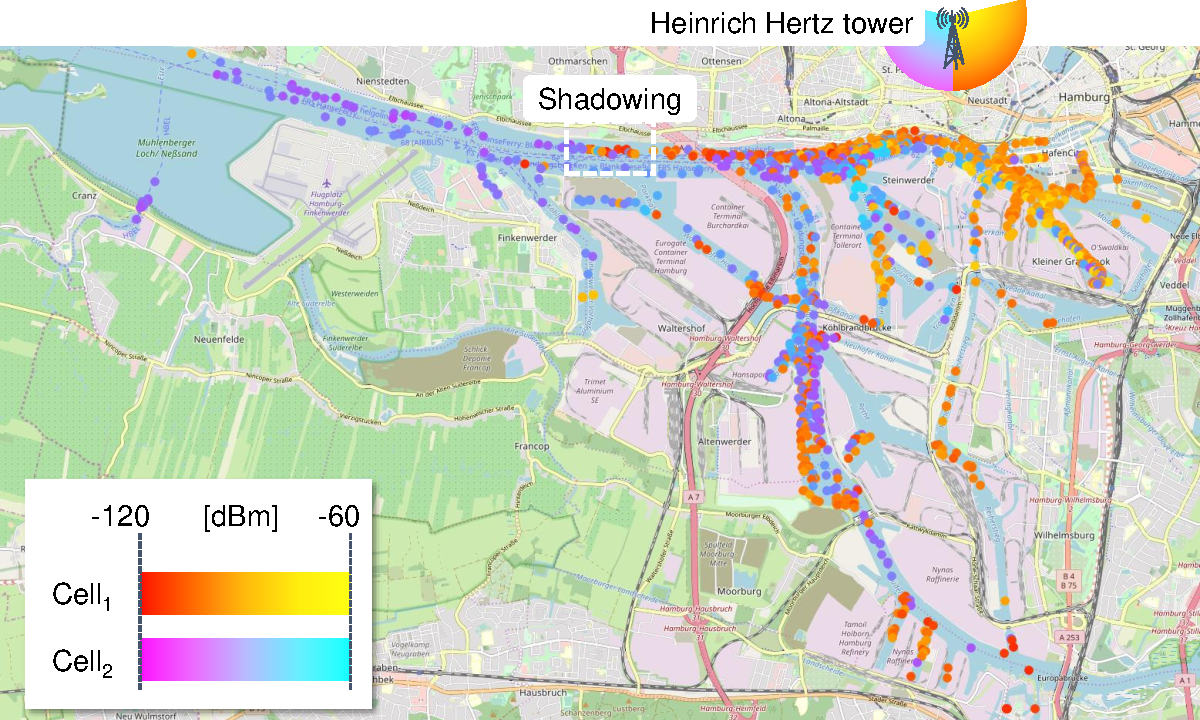
\includegraphics[width=0.8\columnwidth]{figures/10_pred_control/pred_control_testbed/pred_control_testbed.pdf}
				\caption[Smart Seaport 5G testbed map]{Site and collected data from the Smart Seaport 5G testbed.}
				\label{fig:pred_control_testbed}
			\end{figure}
		
			We used this testbed to collect \ac{BTS}-wide \acp{KPI} and \ac{UE} measurements from up to three ships, such as \ac{RSRP} and latency, as well as the ship's position reported by the \ac{GPS}.
			The data collection took place over a time of $6$ months in $5$ second granularity, with all in all around $3$ million records collected.			
			Certain parts of the testbed showed low signal strengths, especially for the ships that were moving around the whole harbor area.
			This was caused partly by the shadowing of the high river bank and tall buildings, and partly simply by the long distances from the \ac{BTS}. 
			An example of such a shadowing effect from the collected \ac{UE} measurements is shown in Fig.~\ref{fig:pred_control_shadowing}: as the ship enters a shadowed area, the \ac{RSRP} droped abruptly and latency increased.
			In the shown example, the shadowing leads to an \ac{RLF}.
			Our goal was to mitigate such shadowing, by reconfiguring the beams dynamically to focus on the shadowed areas when a tracked barge was close to entering these areas.

			\begin{figure}[ht]
				\centering
				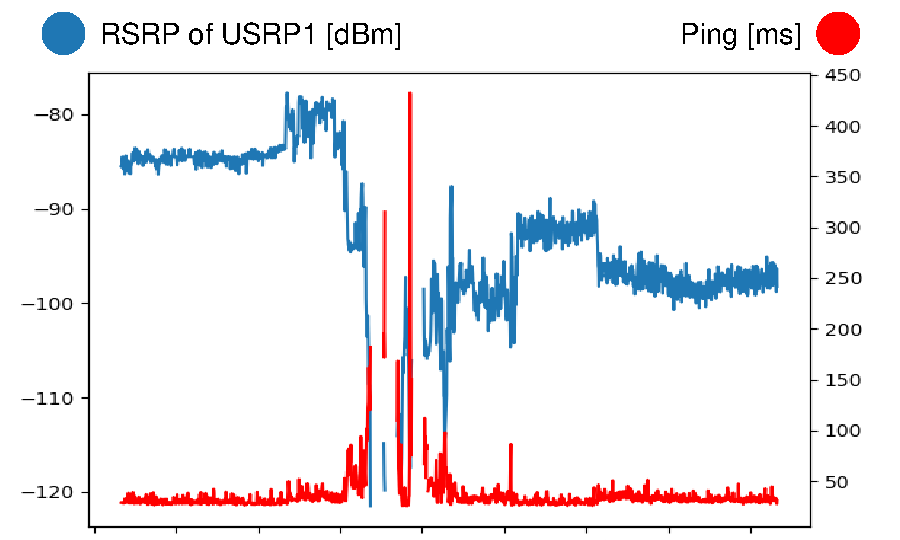
\includegraphics[width=0.5\columnwidth]{figures/10_pred_control/pred_control_shadowing/pred_control_shadowing.pdf}
				\caption[Shadowing effect in the smart seaport dataset]{Shadowing effect experienced by one of the barges.}
				\label{fig:pred_control_shadowing}
			\end{figure}
	
		\subsection{Mobility and QoS Prediction}
	
			Our initial approach studied whether it is possible to use purely analytics and \ac{ML} to predict the above shown service degradations.
			To this end, two \ac{ML} models were created based on the \ac{UE} measurements: a deep \ac{CNN} to predict the movement of the barges (Fig.~\ref{fig:pred_control_models_mobility}), and a shallow \ac{MLP} as a radio propagation map (Fig.~\ref{fig:pred_control_models_rsrp}), to map the predicted locations to radio \ac{QoS}.
			
			\begin{figure}[!ht]
				\centering
				\subfloat[Mobility prediction]{
					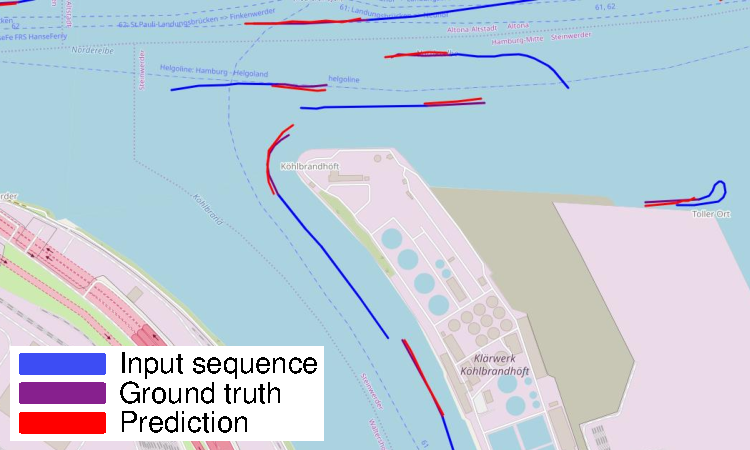
\includegraphics[width=0.48\linewidth]{figures/10_pred_control/pred_control_models/mobility.pdf}
					\label{fig:pred_control_models_mobility}
				}
				\subfloat[Radio propagation map]{
					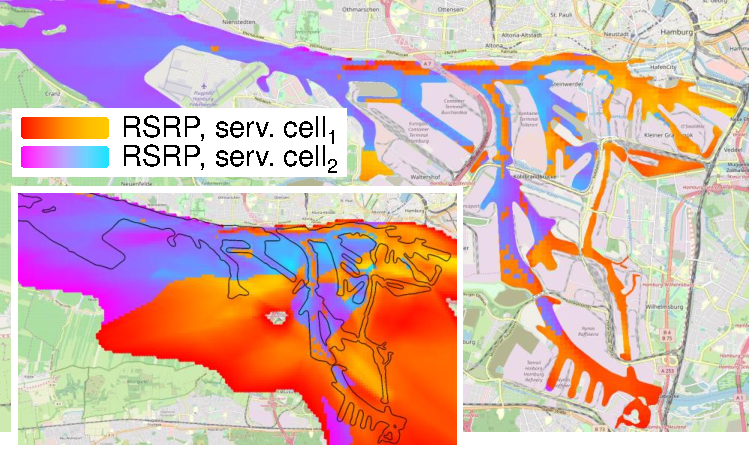
\includegraphics[width=0.48\linewidth]{figures/10_pred_control/pred_control_models/rsrp.pdf}
					\label{fig:pred_control_models_rsrp}
				}
				\caption[MPP and radio map trained on the smart seaport dataset]{Mobility prediction and radio propagation models trained on the testbed data.}
				\label{fig:fig:pred_control_models}
			\end{figure}
			
			The deep \ac{CNN}-based mobility prediction worked excellently.
			The input to the mobility predictor was made up of $32$-long sequences of latitude and longitude coordinates.
			In order to help with the incorporation of inertia-like behavior into the model, we found that it is helpful to extend the input features by also supplying the model with both a per-sequence normalized version of the coordinates, as well as version which contained the differences between individual steps in the sequence.
			With these added features, the mobility predictor was able to predict barge movement quite precisely up to $8$ steps ahead, which corresponds to $40$ seconds into the future.
			
			\begin{figure}[ht]
				\centering
				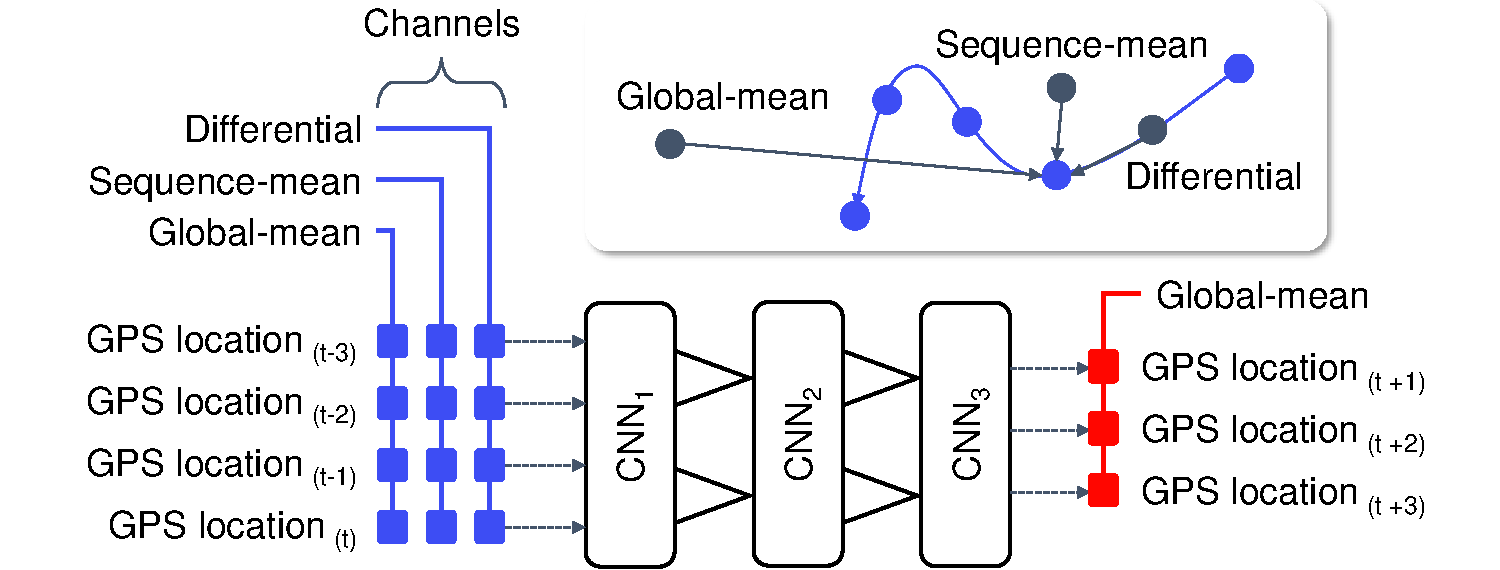
\includegraphics[width=0.85\columnwidth]{figures/10_pred_control/pred_control_cnn/cnn.pdf}
				\caption[Feature engineered inputs for the mobility-predicting CNN]{The feature engineered inputs the the mobility-predicting CNN.}
				\label{fig:pred_control_cnn}
			\end{figure}
			
			Unfortunately, the shallow \ac{MLP} did not function acceptably as a radio propagation map.
			Our reasoning behind using a shallow neural net was to have an inherent regularization and not to overfit the extremely noisy \ac{RSRP} measurements.
			Deeper neural nets tended to learn these noisy observations, forgoing generalization, even if we employed some external regularization scheme, such as weight-decay.
			However, the simple model was not able to properly estimate the radio condition changes with a fine enough granularity.
			Ultimately, it was impossible to find a good trade-off between overfitting and a too simplistic model.			
			We concluded, that for a high-granularity model to be trained, we would have had to collect a lot more data (several magnitudes), which covers basically all the water surface in the harbor.
			However, such data collection, on top of taking a very long time, also requires directed measurement campaigns, as it would have involved areas of the waterways which are not necessarily used during regular operation.			
			This is a general problem for many \ac{ML}-based radio quality models, because they require good quality data, which is only possible to acquire with costly drive-tests.
			However, there is a modern solution to this problem: \emphix{digital twins}{digital twin}, simulated environments updated in real-time to mirror real-world environments.

		\subsection{A Digital Twin for QoS Prediction}
		
			To achieve an accurate mapping between \ac{QoS} and barge locations, we created a digital twin using our proprietary network simulator, focusing on the harbor area.
			The geometric data for the buildings and other occluders -- such as cranes -- were supplied to us by the government of the city of Hamburg.
			After some tuning of the radio propagation parameters and material properties in the simulator, we were able to align the simulation to the recorded measurements from the real testbed, and also reproduce the detected coverage issues.
			Additionally, the simulator was extended to simulate beam forming: in our simulation, each cell was further split into $4$ beams, each of which could be separately controlled by tilting the beam up or down, and setting the transmission power.
			This allowed us to show how the \ac{QoS} predictions, combined with beamforming, could be utilized in closed-loop network automation function to preemptively react to \ac{QoS} degradations.
			The concept was made into a demonstrator, which we named \ac{PLANAR}.
			
			\begin{figure}[ht]
				\centering
				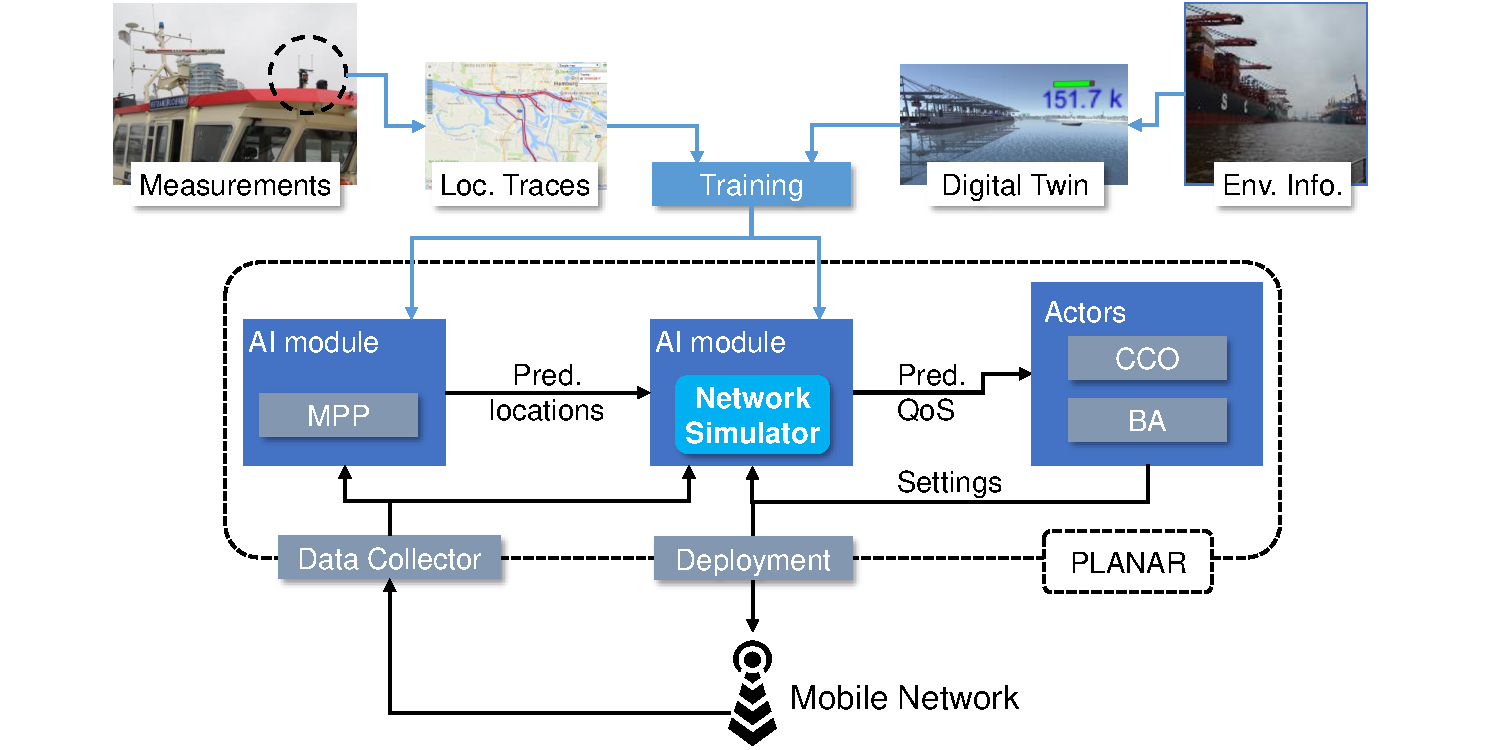
\includegraphics[width=\columnwidth]{figures/10_pred_control/pred_control_architecture/architecture.pdf}
				\caption[PLANAR overview]{The components of PLANAR.}
				\label{fig:pred_control_architecture}
			\end{figure}
			
			The architecture of \ac{PLANAR} is shown in Fig.~\ref{fig:pred_control_architecture}.
			The \ac{MPP} module uses the deep \ac{CNN} to predict barge movement.
			Using the \ac{MPP}'s output as an input to the digital twin, accurate predictions about the barges' \ac{QoS} can be made $40$ seconds into the future.
			The predictions are utilized by optimization actors, which create recommendations for beam reconfiguration.
			In our demonstration, the selected actors are the \ac{CCO}, adjusting cell transmission power, and the \ac{BA} function, optimizing beam tilt.
			The $40$ second prediction window allows for repeated adjustments: the newly set beam configuration is simulated in the digital twin, and if the \ac{RLF} is still present, another round of adjustments can be made.
			\ac{PLANAR} implements the \ac{ML} pipeline concept, as described in \cite{ML5G2019}.
			A video of the demonstrator in action is available online on YouTube\footnote{\url{https://www.youtube.com/watch?v=nMdBbLv2G98}}.
			
		\subsection{Results}

			Out of a total $65206$ sequences, \ac{PLANAR} was able to predict $97.6\%$ that ended in either an \ac{RLF} or below $-120dB$ \ac{RSRP}.
			We encountered altogether $96$ false positives ($0.14\%$ of total observations, and $20\%$ of true drops.
			There were $12$ false negatives ($0.02\%$ of total observations, and $2.5\%$ of true drops).
			In our case, false positives are not dangerous, since the corrective actions are not very intrusive. Also, many of the false positives were very close to our (arbitrary) threshold.
			The false negatives are potentially disruptive, but these were very few.

			An excerpt from the demonstrator shows how the \ac{CCO} and the \ac{BA} functions can prevent predicted degradations (Fig.~\ref{fig:pred_control_example}).
			The dark blue line is the \ac{RSRP} measured by a ship and the light blue line is the predicted value.
			At point $62$ a \ac{RLF} is predicted.
			The \ac{CCO} preemptively adjusts the cell transmission power, and the \ac{BA} function configures the beamforming, so that when the ship is entering the shadowed area, a beam is already pointed there.
			If necessary, the \ac{BA} function will also split a beam to be able to optimally serve the whole covered area.
			With these actions, the ship experiences no degradation at all.
			Once the ships leave the shadowed area, the compensation is gradually configured back to the baseline to save resources and to reduce the compromises the compensating reconfigurations have on other \acp{UE} and slices.
			
			\begin{figure}[ht]
				\centering
				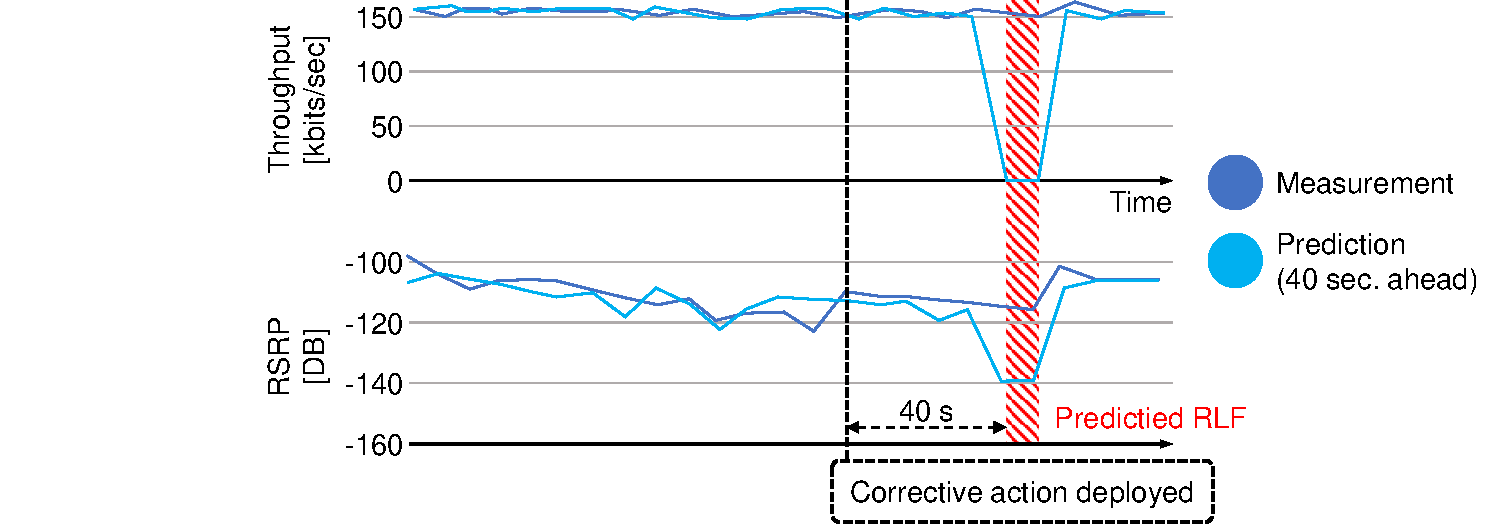
\includegraphics[width=\columnwidth]{figures/10_pred_control/pred_control_example/example.pdf}
				\caption[Example of a beam reconfiguration in PLANAR]{Example of a beam reconfiguration in PLANAR avoiding a RLF.}
				\label{fig:pred_control_example}
			\end{figure}
			
			A further consideration is the robustness of the \ac{ML} models against changes in the environment, including those based on the insights coming from the model itself.
			The advantage of separately predicting the future location and the expected \ac{QoS} using two independent models, is that the reconfigurations only affect the radio propagation model, but not the \ac{MPP}.
			Furthermore, utilizing a digital twin for the radio propagation modeling makes the model capable of accurately following such reconfigurations.
			We believe this demonstrates the advantages of a digital twin in operational network optimization.
			Of course, using a digital twin is not without its hurdles: digital twins require extensive information about the simulated scenario (building models), human labor for setup, live data collected from the users and other elements of the network, and considerable computational power to run the simulation in real-time.
			These requirements make digital twins situational, only applicable to limited use cases and scenarios.
			However, if all requirements are present, digital twins can be used to considerably improve the robustness and adaptability of a network.
			
		\subsection{Conclusion}
		
			As we have seen in the previous chapter (Cha.~\ref{cha:pred_ho}), signal-quality-based prediction can be quite unreliable (noisy), and requires strict post-processing to render the predictions usable.
			I suspect one cause of the high variance is the categorical output required from the predictor, however, there is another underlying issue that further adds to the problem.
			Signal quality is suspect to rapid, seemingly random changes due to fading, without which it is mostly governed by user location.
			However, if location is only present in the data as a latent feature, ``hidden'' behind noisy signal quality measurements, it can be hard to extract for \ac{DL} algorithms, thus, the true cause of the changes is never modeled properly.
			
			Location-based prediction solves this problem by explicitly using location as the input to the prediction model.
			Furthermore, detaching location prediction from radio quality mapping allows for different regularization on the two models, so that the high variance in the radio map can be suppressed without affecting the prediction performance.
			\ac{PLANAR} improves this concept further, by using a digital twin as a radio map, as well as a sandboxing environment, in which beam reconfigurations can be tested before being deployed to the real network.
			However, for all this to work, the precise location of each user has to be collected in real-time, which raises concerns for the users' privacy.
		
	\section{On Data Privacy}
		\label{cha:pred_control:sec:privacy}
	
		While the location-based prediction in \ac{PLANAR} solves the issue of high variance seen with signal-quality-based radio environment prediction, it introduces another one.
		The measurement and reporting of signal quality is an integral part of the radio communication in mobile networks, used for the channel equalization in older generations, \ac{OFDM} and \ac{MIMO} in newer ones, as well as for scheduling.
		Thus, a model using signal quality as input for predictions requires basically no extensions on currently available signaling in the network.
		Furthermore, because signal quality is an essential part of radio communication, users of mobile phones inherently ``opt-in'', allowing the network to collect this information about them.
		
		The most common method of user localization is \ac{GPS}, but \ac{5G} also supports diverse user localization methods based on signal quality measurements, with more methods planned for later releases/generations.
		Generally, signal-quality-based triangulation exhibits the same problem as signal-quality-based prediction: the location estimations are usually quite noisy, thus relatively unprecise -- precision ranges from tens of meters to a few meters -- making them generally on par or worse than commercial \ac{GPS} accuracy.
		For industrial applications, some methods' precision can be improved down to a few centimeters with strategically placed access points.
		The collection of the user's location is of high interest: within the mobile network, user location can be used for network planning, \ac{MDT}, or predictive reconfiguration as in \ac{PLANAR}, while applications using the mobile network -- such as food delivery apps or taxi services -- can use it to find the user.
		But herein lies the problem: user location is a very sensitive information, which can be used for malicious intent in many ways if it falls into the wrong hands.
		Because of this, user location reporting is a highly controlled feature, where users have to strictly opt-in for it to work.
		
		\ac{PLANAR} and similar smart radio concepts are planned for industrial customers and smaller campus networks, where functionality depends on \ac{URLLC}.
		In these scenarios, user localization is a non-issue, as the users also inherently opt-in to reporting their locations.
		Everyday mobile phone users usually do not need or expect high reliability from the mobile network, thus, for them location-based features are only interesting on the application-level.
		However, there is a growing number of potential applications which would use the commercial networks, but require \ac{URLLC}: remote controlled, or self-driving vehicles (cars or drones), used for personal transport or deliveries.
		In these use cases, high reliability is a necessity for some of features, such as collision avoidance, platooning or remote control, which is believed to be only feasible with adaptive smart radio solutions, such as \ac{PLANAR}.
		However, the collection of user location might cause the same problems in these scenarios as for mobile phone users, for example: travelers in self-driving taxis could be tracked, or delivery drones transporting valuable packages could be intercepted.
		
		We have devised a location-based predictive handover mechanism, called \ac{PACHO}, which tries to solve this problem.
		The key idea in \ac{PACHO} is that the predictive model is run on the \ac{UE} itself.
		This way, the user location does not have to be communicated over the network, saving signaling overhead, and also avoiding privacy issues.
		The complete life cycle of a \ac{PACHO} model can be seen in Fig.~\ref{fig:pred_control_pacho}.
		In the case of \ac{PACHO}, instead of the location of the user, derived information is communicated over the network, which is not privacy sensitive.
		An early idea was for the \ac{PACHO} model to directly output handover triggers, similarly to the output in the predictive handover concept (Cha.~\ref{cha:pred_ho}), however, this approach is problematic for two reasons.
		First, in mobile networks, \acp{UE} generally do not make control decisions, only report measurements, and the network is the one scheduling, triggering handovers, assigning cloud resources, etc.
		A \ac{PACHO} model directly triggering handovers would have broken this rule.
		Second, we suspect the categorical outputs required for direct handover triggers do not function great with \ac{DL} models, causing noisy, high variance outputs, as shown previously (Cha.~\ref{cha:pred_ho}).
		Instead, in the final \ac{PACHO} concept, the model recommends \ac{CIO} and \ac{TTT} values to the network, which influence handover decisions in a more semi-indirect manner.
		This approach has multiple advantages: the model outputs can be easily sanitized by restricting the values to an acceptable range, the network can overrule the recommendations, and the whole system can fall back to legacy \ac{CIO} and \ac{TTT} optimization schemes if the \ac{UE} dos not support this feature.
		
		\begin{figure}[ht]
			\centering
			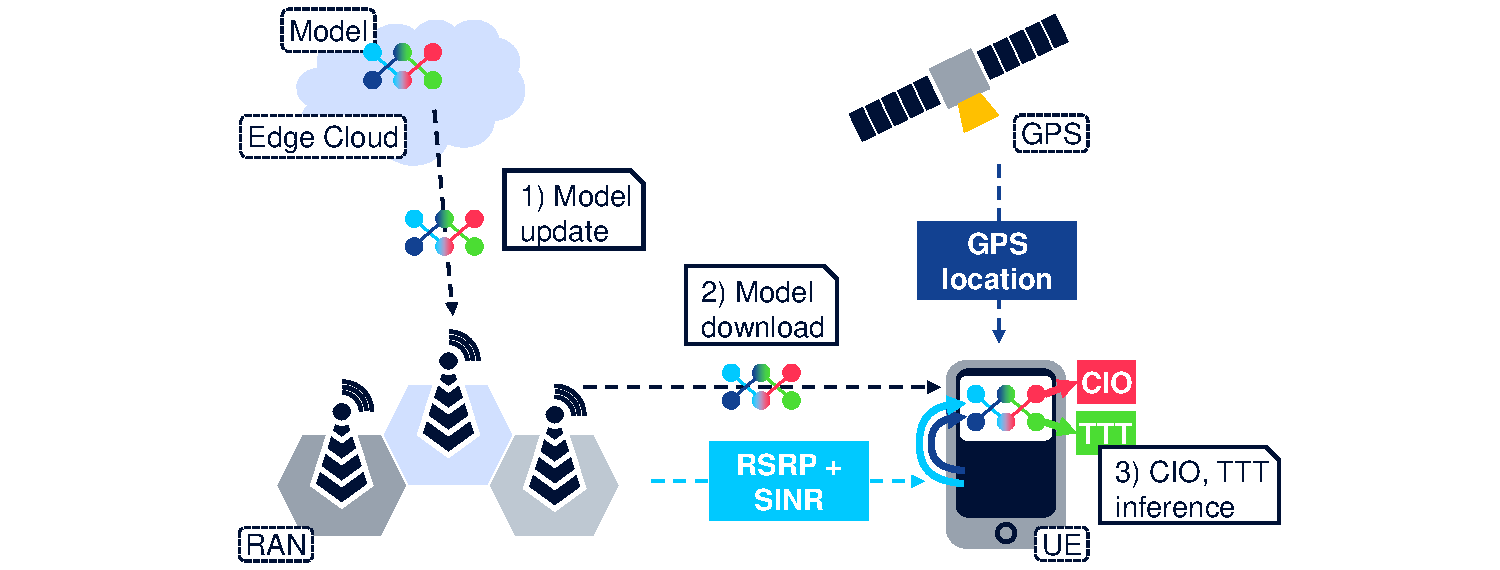
\includegraphics[width=\columnwidth]{figures/10_pred_control/pred_control_pacho/pacho.pdf}
			\caption[The PACHO model life cycle]{The PACHO model life cycle.}
			\label{fig:pred_control_pacho}
		\end{figure}
		
		Some problems still remain with \ac{PACHO}.
		Naturally, training or refreshing the model should still be done in the network using collected user locations, which might require some form of ``benefit'' for the user as an opt-in incentive.
		For increased privacy, we have devised a randomized data collection method, where location information is anonymized, encrypted and collected with a random delay, to hide the user's identity as best as possible.
		The reporting also consumes excess power from the device, which limits battery life.
		Another consideration is the power consumption when inferring with these models: most modern mobile \acp{CPU} include some form of hardware acceleration for \acp{DNN}, making the calculations a little more power efficient.
		However, \ac{DNN} inference still requires an excess of power, which often limits the mobile devices' uptime to a handful of minutes before needing a recharge, thus also limiting the usability of the feature.
		In order to save battery life, for both reporting and inference we have devised a dynamically changing reporting/updating frequency mechanism, with which users far from cell edges only report or infer infrequently, while users close to cell edges more frequently.
		If we can overcome these obstacles, \ac{PACHO} could be theoretically deployed for any consumer, even in a large-scale commercial mobile network, making the widespread use of \ac{URLLC} feasible.
		Unfortunately, the \ac{PACHO} concept has not been scientifically evaluated yet, although we plan to start experimentation in the near future.

		Deep learning often requires data that is invasive: facial recognition requires photos of people, speech recognition requires audio recordings, and mobility prediction requires user location to be collected.
		I believe that for the widespread acceptance of \ac{DL} and the removal of skepticism developed around it, it is of utmost importance that the privacy of the users is respected.
		Any mechanism that collects sensitive information should make all reasonable effort at hiding the identity of the person(s), and should explicitly ask the user's permission if sensitive data is collected.
		Only if we don not have to worry about our privacy is when \ac{DL} can truly improve our lives.
